\documentclass{sig-alternate-10pt}

\newcommand{\ttt}{\texttt}

\usepackage{graphicx}
\usepackage{changepage}
\usepackage{lipsum}
\usepackage{booktabs}

\title{FLASH\\Fast Linux Advanced Scheduler Hardware}
\author{
	Mark Aligbe \\
	    \email{ma2799@columbia.edu}
	\and
    Chae Jubb \\
        \email{ecj2122@columbia.edu}
}
\date{4 May 2015}

\begin{document}
\maketitle

\begin{abstract}
As accelerators become more common and necessary as a way to continue Moore's Law in the absence of Dennard Scaling, researchers explore segments of computation that can be improved with the aid of dedicated hardware. This paper presents FLASH, a hardware scheduler to take over the task of scheduling from the operating system. FLASH is able to make scheduling decisions in much fewer cycles as compared to modern operating system schedulers. The scheduling decisions it makes are just as good as those that would be made in software, but in much reduced time and without negatively impacting processor performance features. FLASH is designed to keep kernel modifications minimal, only requiring changes when the kernel scheduling interface changes.

\end{abstract}


\section{Introduction}
\label{sec:intro}
\lipsum[1-3]


\section{Scheduling in the Kernel}
\label{sec:sched_in_kernel}
% Mark
\subsection{History of Linux Schedulers}
\subsection{Implementation of CFS}
\subsection{Limitations}


\section{Related Works}
\label{sec:related_works}
Previous hardware scheduling units focus completely on embedded systems with
a fixed number of tasks each with fixed priority
\cite{kuacharoen2003configurable, morton2004hardware, nacul2007hardware, nakano1995hardware,
park2008hardware}.  Scheduling under these fairly restrictive constraints is
greatly simplified with respect to desktop scheduling as there is a much
more defined ordering between tasks.

Additionally, there is often a small number of tasks relative to a desktop
environment.  This means that much simpler algorithms may be used in an
attempt to approximate the optimal task ordering.

The major novel challenge in escalating to a desktop Linux is handling the
dynamic, unbounded (from a realistic hardware perspective) number of tasks.
The initial FLASH prototype addresses this in an unsatisfying way: by
arbitrarily fixing the number of tasks that can be managed with its
scheduling policy.  As discussed in detail in Section~\ref{sec:future},
future iterations will remove this restriction by reserving a small section
of memory.

Because we aim to support an unbounded number of tasks, we must implement
a scheduler comparable to the default CFS currently used by the kernel.
While a simpler implementation than the kernel default, the FLASH scheduler
is implemented in accordance with the major principle of CFS
\cite{wong2008cfs}.

We should also consider the architecture of previous hardware schedulers.
Many of the previously cited works were designed either as ASICs
(Application Specific Integrated Circuits) or on FPGAs (Field Programmable
Gate Arrays) rather than a general purpose CPUs.  This makes scheduling of
resource usage slightly different in that there is not always an overhead of
a context switch: we may simply be deciding which process can use
a particular multiplier.


\section{FLASH Architecture}
\label{sec:arch}
% Chae
\lipsum[1-8]


\section{Integration}
\label{sec:integration}
% intro stuff here
\subsection{Cyclone V}
% Mark
\begin{figure}
	\begin{center}
		%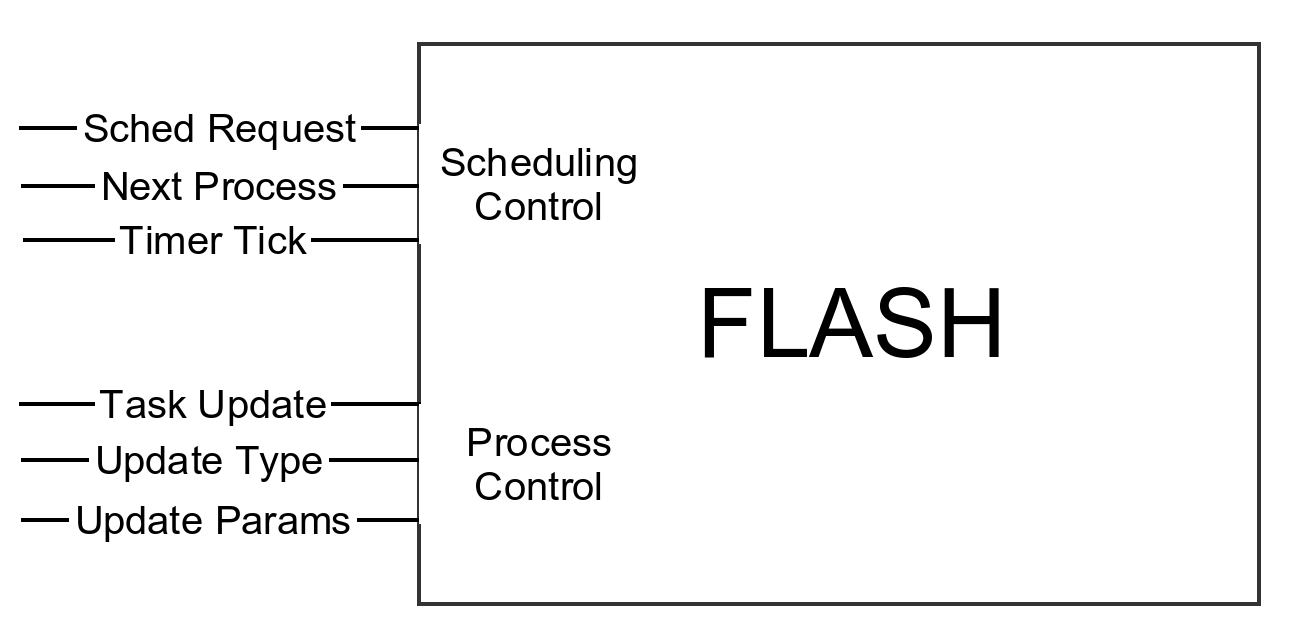
\includegraphics[width=0.65\textwidth]{fig/flash-diagram.png}
		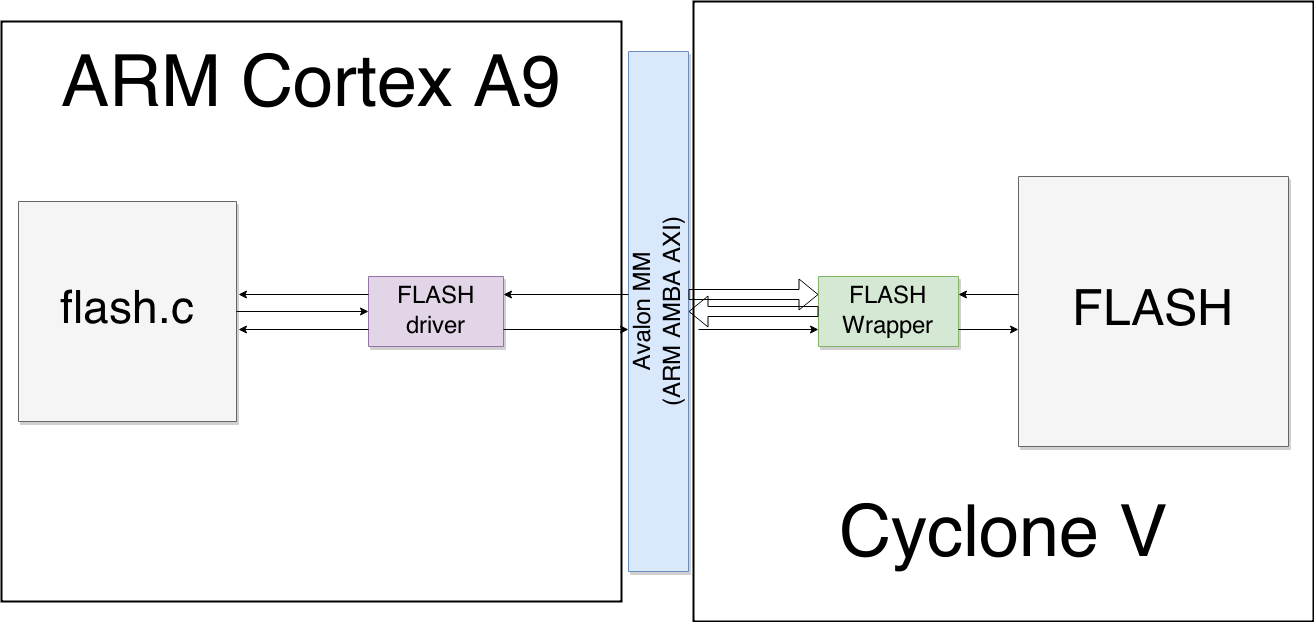
\includegraphics[width=0.9\linewidth]{fig/sockit-architecture.png}
		\caption{
			FLASH System Architecture: Interface.  Note the distinction between
			the \emph{Process Control} and \emph{Scheduling Control} Interfaces.
		}
		\label{fig:sockit_overview}
	\end{center}
\end{figure}


\subsection{Kernel mods}
% Chae
\lipsum[1-3]


\section{Applications}
\label{sec:apps}
% Mark
\lipsum[1-3]


\section{Engineering Experiences}
\label{sec:eng_exp}
% both
\lipsum[1-3]


\section{Conclusion}
\label{sec:conclusion}
\lipsum[1]

\nocite{*}
{
	\bibliographystyle{abbrv}
	\bibliography{ref}
}

\end{document}
